% ══════════════════════════════════════════════════════════════════
% PAGE DE GARDE — modèle ENASTIC (fragment, inclus par main.tex)
% ATTENTION : chaque \begin{...} doit avoir son \end{...}
% ══════════════════════════════════════════════════════════════════

\begin{titlepage}
	\thispagestyle{empty}
	
	% ── Bordure bleue extérieure ──────────────────────────────────────
	\begin{tikzpicture}[remember picture, overlay]
		\draw[bleuENASTIC, line width=1.6pt]
		([xshift=0.9cm,  yshift=-0.9cm] current page.north west) rectangle
		([xshift=-0.9cm, yshift=0.9cm]  current page.south east);
	\end{tikzpicture}
	
	% ── Logo ENASTIC ──────────────────────────────────────────────────
	\noindent
	\IfFileExists{images/logo_enastic.png}{%
		
\includegraphics[width=6cm]{images/logo_enastic.png}%
	}{%
		{\Large\bfseries\color{bleuENASTIC}ENASTIC}\\[2pt]
		{\footnotesize École Nationale Supérieure des TIC}%
	}
	
	\vspace{1.6cm}
	
	% ── Titre principal ───────────────────────────────────────────────
	\begin{center}
		{\fontsize{28}{34}\selectfont\bfseries Projet de Fin d'Études}
		
		\vspace{1cm}
		
		{\large En vue de l'obtention du Diplôme de Licence en Informatique}
		
		\vspace{0.5cm}
		
		{\large \textbf{Option} : Informatique}
		
		\vspace{1.4cm}
		
		% ── Encadré THÈME (coins arrondis bleus) ──────────────────────────
		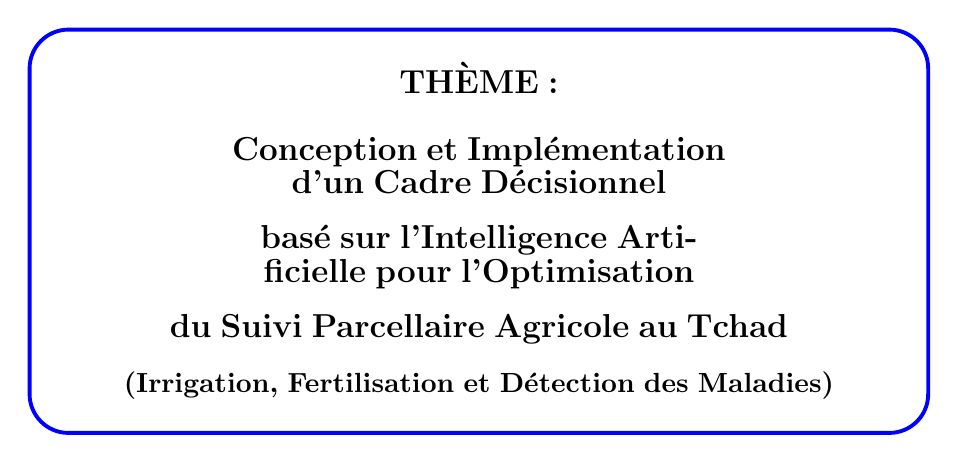
\begin{tikzpicture}
			\node[draw=blue, line width=1.4pt, rounded corners=14pt,
			inner xsep=14pt, inner ysep=12pt,
			text width=0.86\textwidth, align=center]{%
				{\large\textbf{THÈME :}}\\[12pt]
				{\large\bfseries
					Conception et Implémentation d'un Cadre Décisionnel}\\[8pt]
				{\large\bfseries
					basé sur l'Intelligence Artificielle pour l'Optimisation}\\[8pt]
				{\large\bfseries
					du Suivi Parcellaire Agricole au Tchad}\\[8pt]
				{\bfseries (Irrigation, Fertilisation et Détection des Maladies)}%
			};
		\end{tikzpicture}
	\end{center}
	
	\vspace{1.4cm}
	
	% ── Rédigé par / Sous la Direction de ─────────────────────────────
	\noindent
	\begin{minipage}[t]{0.46\textwidth}
		\underline{\textbf{Rédigé et Présenté par}} :\\[10pt]
		TOURABI ISSAK HISSEIN
	\end{minipage}
	\hfill
	\begin{minipage}[t]{0.50\textwidth}
		\underline{\textbf{Sous la Direction de}} :\\[10pt]
		Dr. MOUAZ MIKAIL,\\
		Enseignant Chercheur à ENASTIC
	\end{minipage}
	
	\vspace{1.6cm}
	
	% ── Jury ──────────────────────────────────────────────────────────
	\begin{center}
		\underline{\textbf{Jury}} :\\[8pt]
		\ldots\ldots\ldots\ldots\ldots\ldots\ldots\ldots\ldots\ldots\ldots
		\ldots\ldots\ldots\ldots\ldots\ (Président)\\[6pt]
		\ldots\ldots\ldots\ldots\ldots\ldots\ldots\ldots\ldots\ldots\ldots
		\ldots\ldots\ldots\ldots\ldots\ (Rapporteur)
	\end{center}
	
	\vfill
	
	% ── Année académique dans une ellipse ─────────────────────────────
	\begin{center}
		\begin{tikzpicture}
			\node[draw=black, line width=0.9pt, ellipse,
			inner xsep=18pt, inner ysep=6pt]
			{\textbf{Année Académique 2025--2026}};
		\end{tikzpicture}
	\end{center}
	
\end{titlepage}